\documentclass[a4paper,titlepage,10pt]{article}
\usepackage[margin=0.7in]{geometry}
\usepackage[spanish]{babel} % Le indicamos a LaTeX que vamos a escribir en espa�ol.
\usepackage[latin1]{inputenc} % Permite utilizar tildes y e�es normalmente
%\usepackage{framed}
\usepackage{caratula}
\usepackage{verbatim}

\titulo{Trabajo Pr�ctico 1\\Carpooling}
\fecha{19 / 09 / 2012}
\materia{Ingenier�a De Software 1}
\grupo{Grupo 1}
\integrante{Browarnik, Mart�n}{LIBRETA/10}{mibrowar0@gmail.com}
\integrante{Carreiro, Mart�n}{45/10}{martin301290@gmail.com}
\integrante{Kujawski, Kevin}{459/10}{kevinkuja@gmail.com}
\integrante{Ortiz de Zarate, Juan Manuel}{LIBRETA/10}{jmanuoz@gmail.com}
\integrante{Soifer, Alexis}{LIBRETA/10}{alex1879@gmail.com}
\begin{document} 

\maketitle

\section{Aclaraciones} %Decisiones tomadas por el grupo

\subsection{Calificaciones} %Agregra una subseccion por tema
\begin{itemize}
\item Un viaje es un recorrido instanciado seg�n una fecha. Es decir, el recorrido indica qu� d�as se va a realizar, y el sistema detecta cuando se cumpli� otro per�odo del recorrido y crea un viaje.
\item Una calificaci�n se asigna a un conductor a partir de un viaje.
\item La calificaci�n del viaje indica si el mismo se realiz� o no
\end{itemize}

\subsection{Retribuciones} %Agregra una subseccion por tema
\begin{itemize}
\item Un viaje se considera pago cuando los pasajeros y el conductor informaron que pagaron y recibi� el pago respectivamente.
\end{itemize}

\newpage

\section{Diagrama de Contexto} %Poner imagenes de contexto

\begin{center}
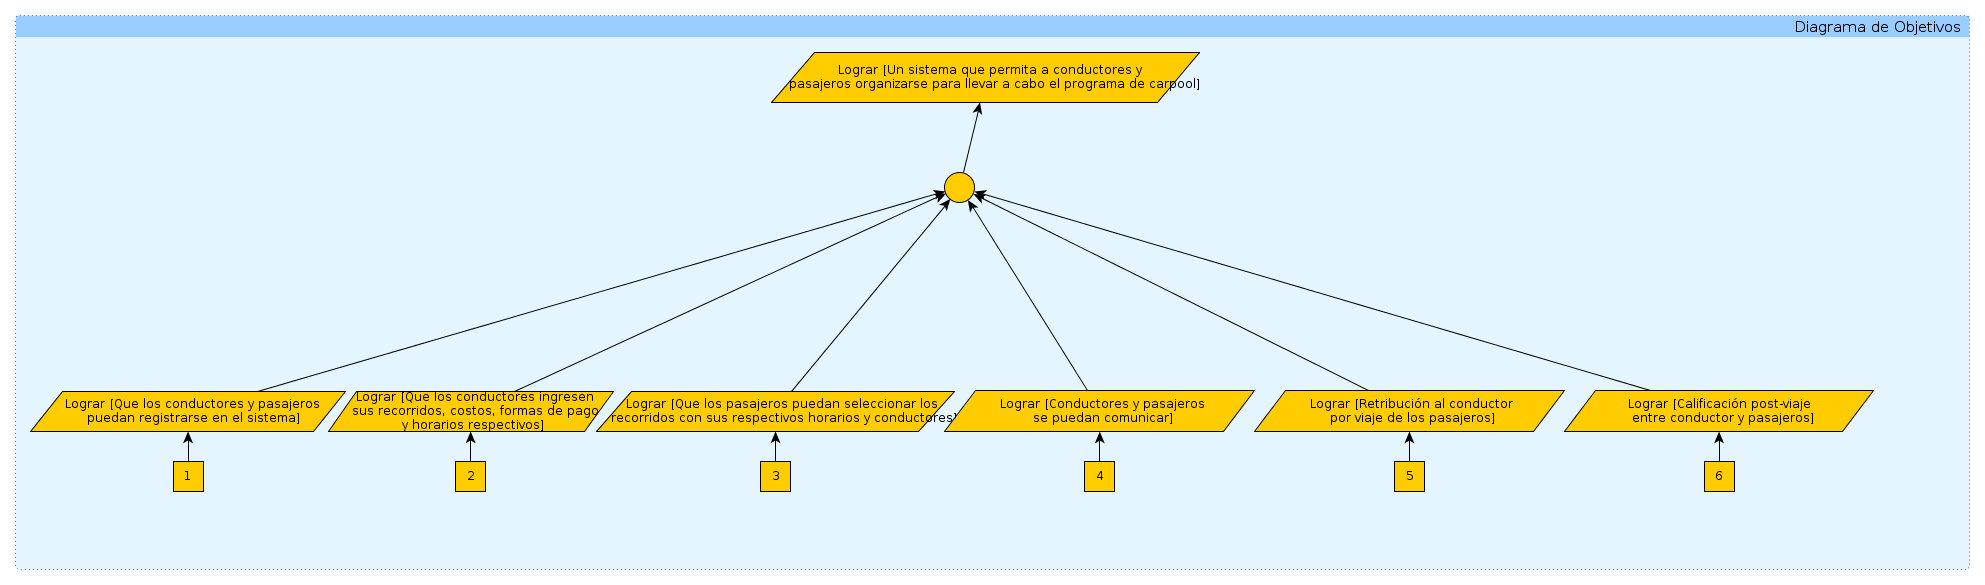
\includegraphics[height=7cm,width=19cm]{imagenes/Diagramaobjetivos.png}
\end{center}

\newpage

\section{Diagrama de Objetivos} %Poner imagenes de objetivos

\newpage

\section{Escenarios} %Escribir los escenarios
Aqu� detallaremos algunos de los posibles escenarios del sistema de Carpooling

\subsection{Escenario 1: Algo}

\end{document} %Termin�!

